\documentclass[stu,12pt,floatsintext]{apa7}
% \documentclass[stu,12pt,floatsintext]{apa6}


% ============ Required Packages ============
\usepackage[english]{babel}  % Provides language-specific definitions
\usepackage[utf8x]{inputenc}  % Allows use of non-ASCII characters
\usepackage{amsmath,amssymb}  % Advanced math formatting
\usepackage{graphicx}  % Required for inserting images
\usepackage[colorinlistoftodos]{todonotes}  % Todo notes for draft versions
\setlength{\marginparwidth}{2cm}  % Set the margin width for todo notes
\usepackage{apacite} 
\usepackage{natbib}  % Provides citation commands
\bibliographystyle{apacite}  % APA citation style

% ============ Document Metadata ============
\title{\Large{Template and Sample for Writing APA 7 Manuscripts with Bibliography}}
\shorttitle{APA LaTeX Template}  % Required for running headers
\author{First Last}
\affiliation{Department name \\ Organization name}
\date{\today}  % Automatically inserts current date

% ============ Abstract ============
\abstract{
    The abstract should be a single paragraph of 150-250 words.\\
    % It should include:
    % - Research problem/purpose
    % - Method
    % - Results
    % - Conclusions/implications
This document serves as a comprehensive template for creating APA-style manuscripts using LaTeX. It demonstrates proper formatting for various sections, including figures, tables, citations, and references. The template is compatible with both APA6 and APA7 styles and features extensive documentation and examples. Users can easily adapt this template by replacing sample content with their own research material while maintaining APA compliance.
}

% ============ Main Document ============
\begin{document}
\maketitle

% ============ Introduction Section ============
\section{Introduction}
The introduction should:
\\- Present the research problem and its context
\\- Review relevant literature
\\- State research questions/hypotheses
\\- Outline the paper's structure



To \textbf{bold text}, \textit{italic text}, \textbf{\textit{italic and bold text}}, 
\underline{underlined text}, \underline{\textit{italic and underlined text}}, 
\underline{\textbf{bold and underlined text}}, 
\underline{\textbf{\textit{italic, bold, and underlined text}}}, \textsc{small caps text}, \texttt{typewriter text}, 
\emph{emphasized text}, {\Large large text} (e.g., large, small, tiny, etc.).


% Example of citation usage:
To cite papers, use various citation commands:
\begin{itemize}
    \item Regular citation: \cite{mujtaba2023frc}
    \item Author as part of sentence: \citet{mujtaba2024ff}
    \item Multiple citations: \citep{mujtaba2023frc, mujtaba2024ff}
\end{itemize}

% Example of research question formatting:
\begin{quote}
\textit{How do structured templates influence the quality of research manuscripts?}
\end{quote}

% ============ Methodology Section ============
\section{Methodology}
This is the methodology section to describe the approach.

\subsection{Analysis}

% ============ Example of figure insertion ============
\begin{figure}[ht]
    \centering
    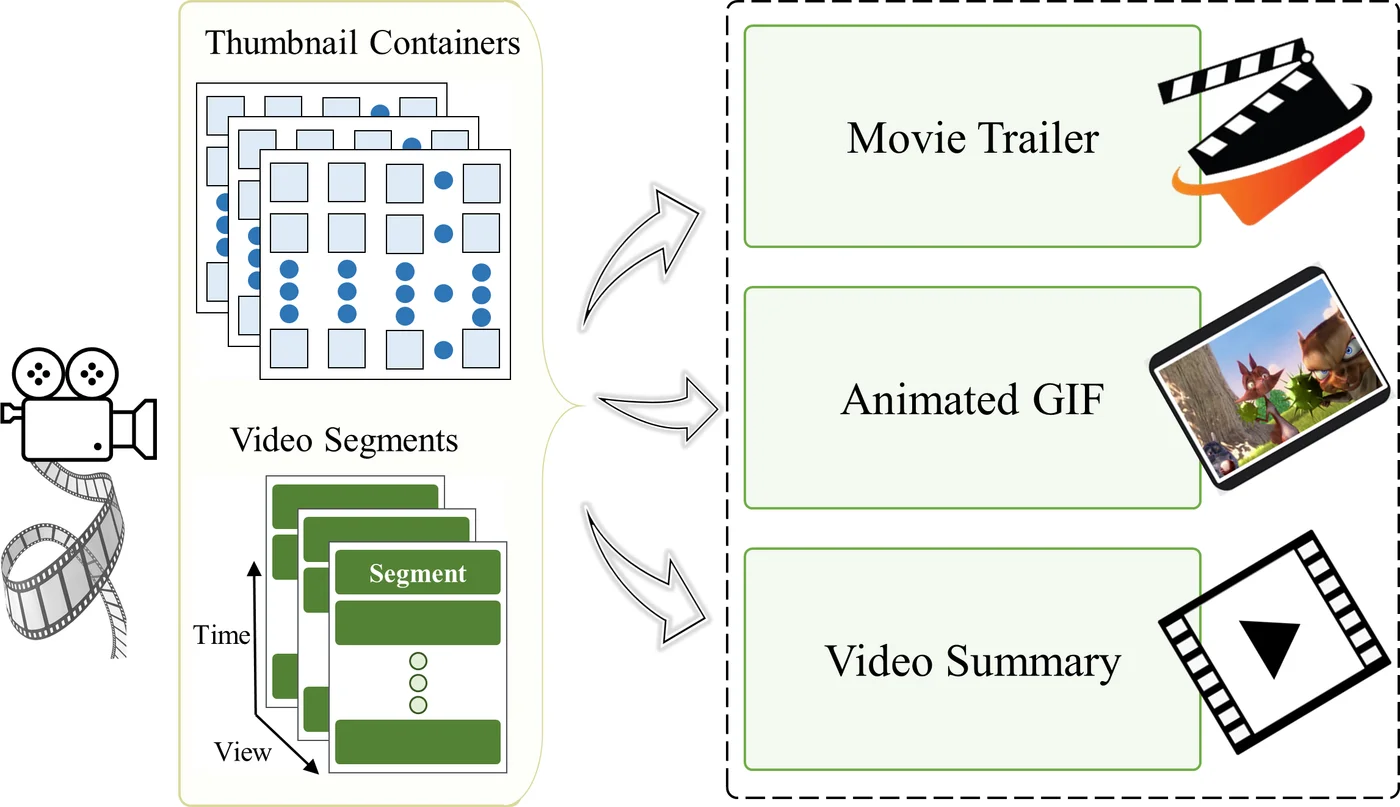
\includegraphics[width=0.75\linewidth]{figures/sample_img.png}
    \caption{Sample figure caption.}
    \label{fig:writing_scores}
\end{figure}

% ============ Example of figure insertion with scale ============
\begin{figure}[ht]
    \centering
    % Scale the image by a factor of 0.3
    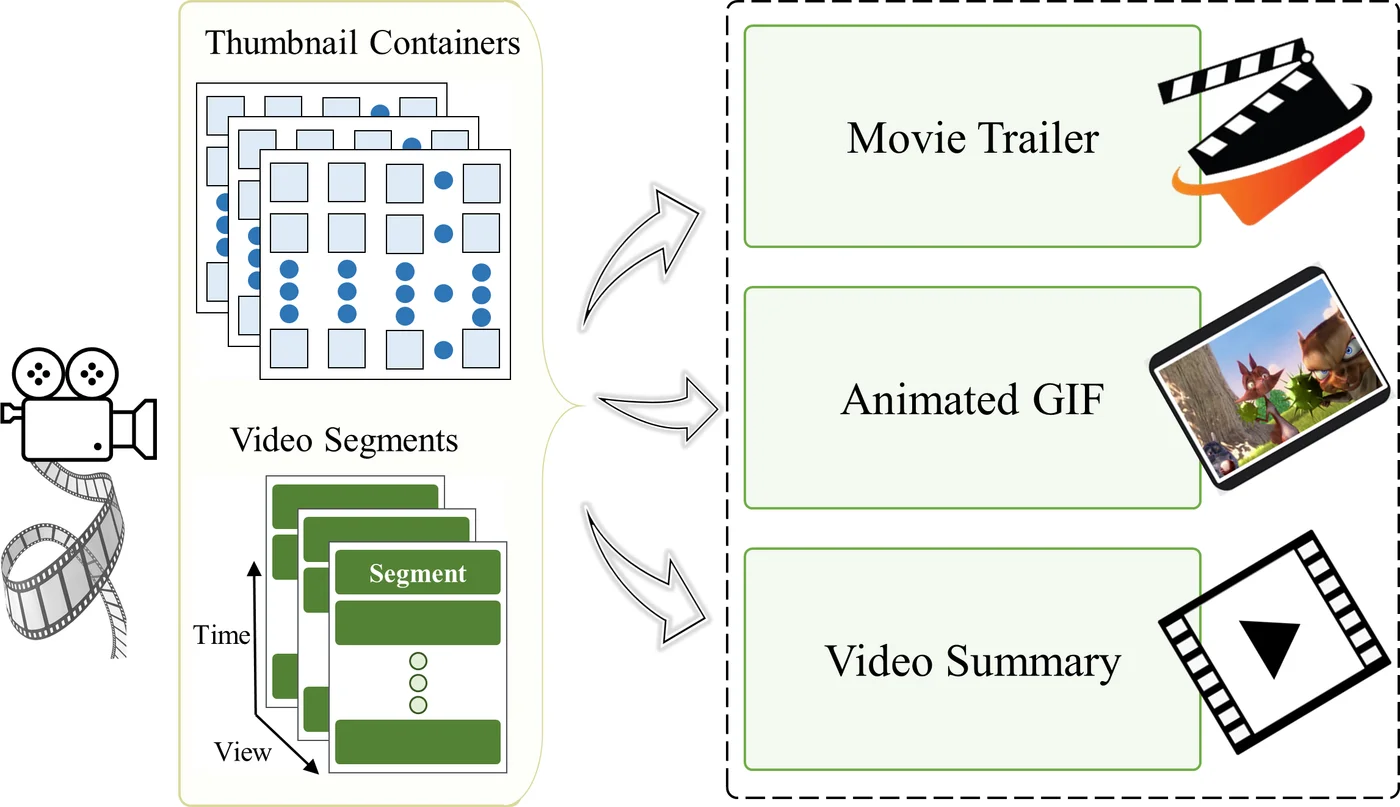
\includegraphics[scale=0.3]{figures/sample_img.png}
    \caption{Sample figure with scaling.}
    \label{fig:scaled_sample}
\end{figure}


% ============ Example of figure insertion with rotation and size ============
\begin{figure}[ht]
    \centering
    % Rotate the figure 90 degrees and set the width to 0.5 of the text width
    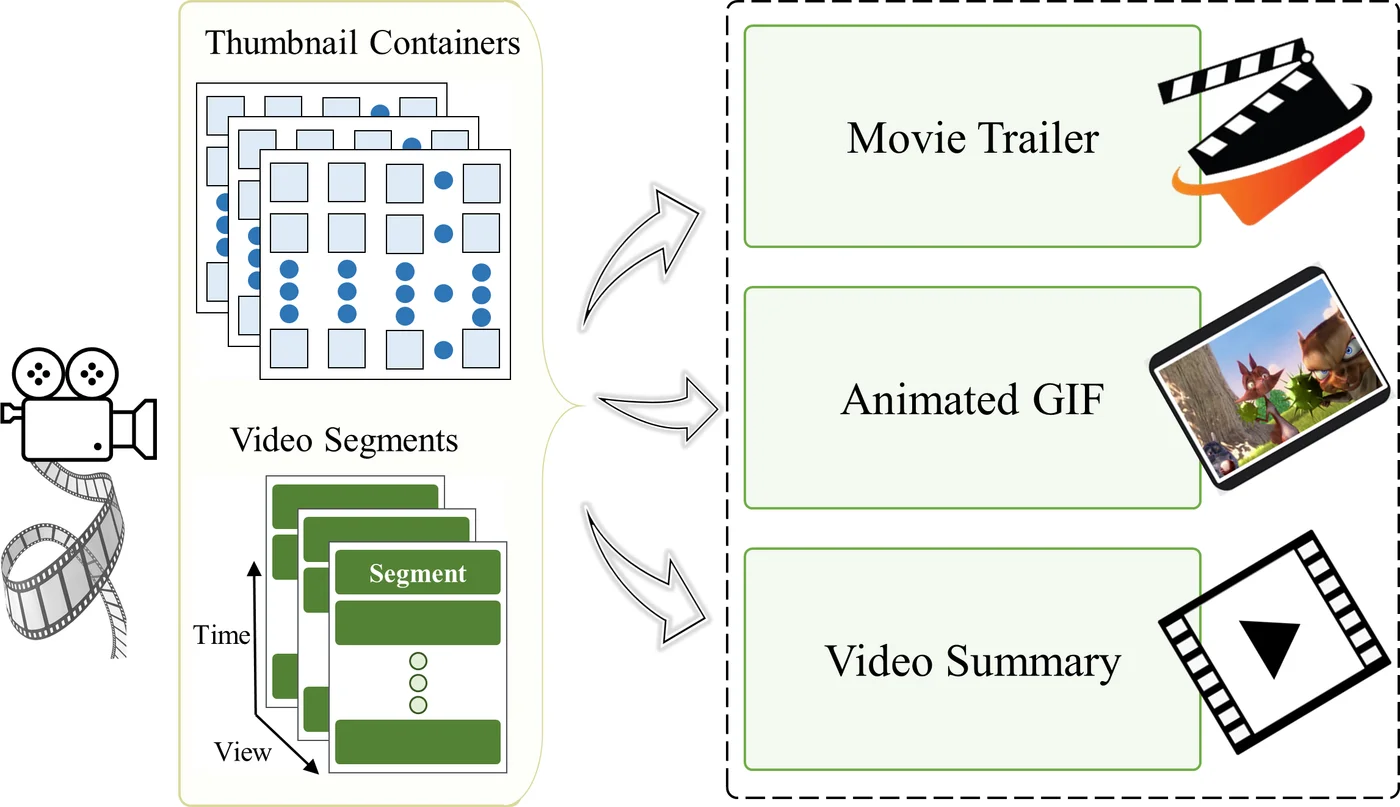
\includegraphics[angle=90, width=0.5\linewidth]{figures/sample_img.png}
    \caption{Sample figure with rotation and resized.}
    \label{fig:rotated_sample}
\end{figure}


Example of figure insertion with t, h, and !b positioning 

% ============ Example of figure insertion with t, h, and !b positioning ============
\begin{figure}[!b]
    \centering
    % Rotate the figure 90 degrees and set the width to 0.5 of the text width
    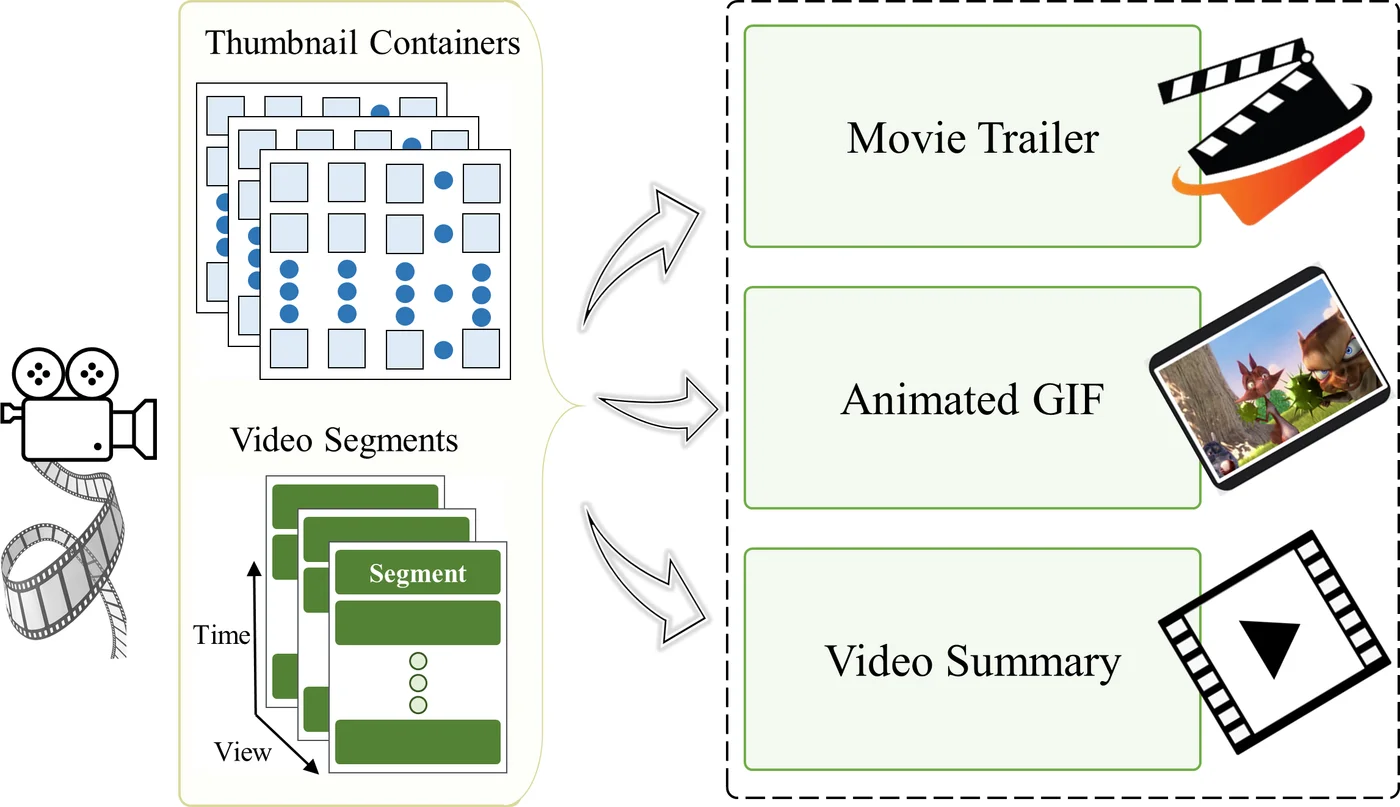
\includegraphics[angle=90, width=0.5\linewidth]{figures/sample_img.png}
    \caption{Sample figure with forced bottom placement and rotation.}
    \label{fig:sample_figre}
\end{figure}



\begin{figure}[!ht]
    \centering
    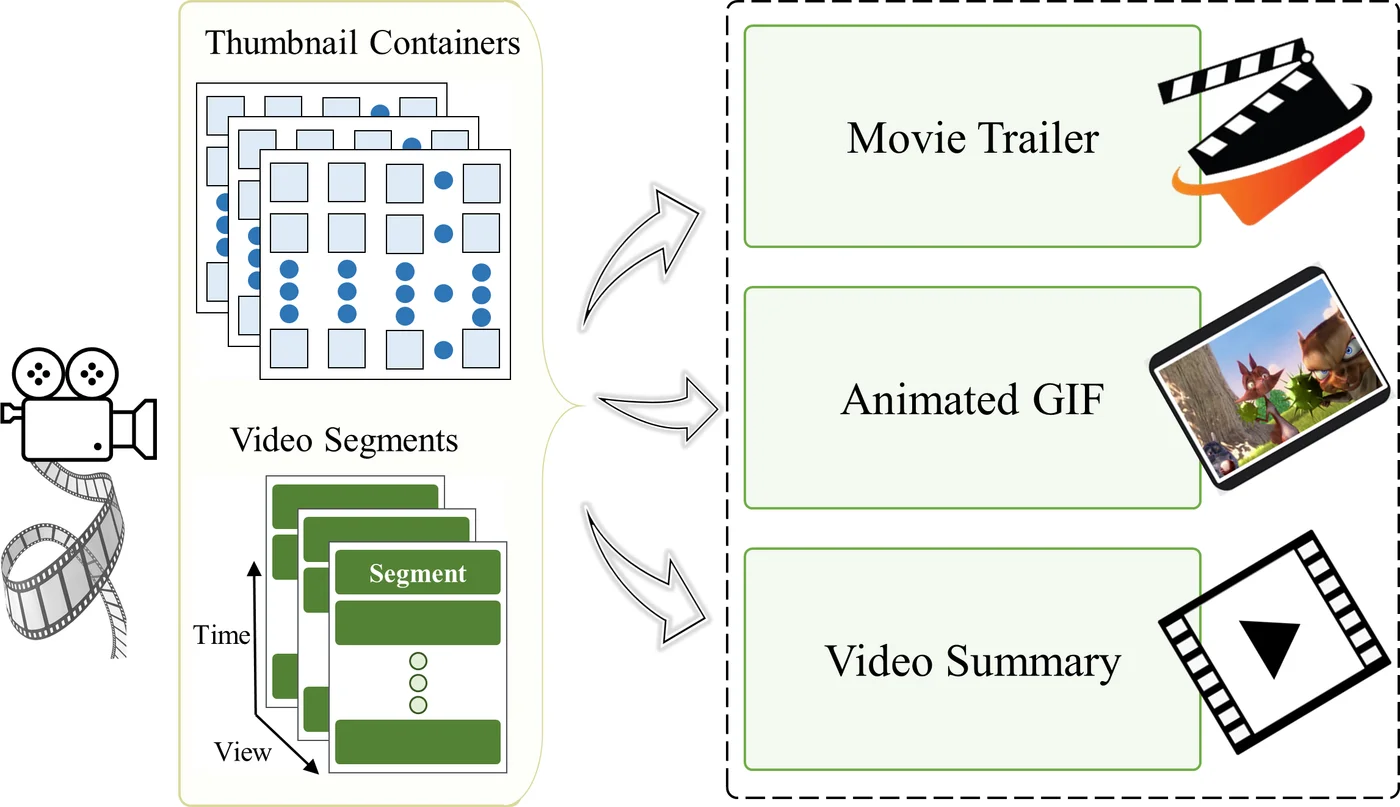
\includegraphics[width=0.6\linewidth]{figures/sample_img.png}
    \caption{Sample figure with forced placement at here or top.}
    \label{fig:sample_figure}
\end{figure}

% ============ Results Section ============
\section{Results}
% Present findings in a logical order:
% - Descriptive statistics first
% - Inferential statistics second
% - Include tables and figures as needed

\subsection{Descriptive Statistics}
% Example of table creation
\begin{table}[ht]
    \caption{Descriptive of the table}
    \centering
    \begin{tabular}{lcc}
        \hline
        Type &  Column Two & Column Two \\
        \hline
        Value one & 000 & 00.0 \\
        value two & 000 & 00.0 \\
        \hline
    \end{tabular}
    \label{tab:descriptive_stats}
\end{table}





% ============ Discussion Section ============
\section{Discussion and Conclusions}
% Include:
% - Summary of findings
% - Interpretation of results
% - Limitations
% - Future research directions
% - Practical implications

Our results align with previous research \citep{mujtaba2023frc}. This suggests several key points:

\begin{itemize}
    \item one
    \item two
    \item three
\end{itemize}

% ============ References Section ============
\bibliography{references}

\end{document}
